\subsection{SGX Memory Access Protection}
\label{sec:sgx_access_protection}

SGX guarantees that the software inside an enclave is isolated from all the
software outside the enclave, including the software running in other enclaves.
This isolation guarantee is at the core of SGX's security model.

It is tempting to assume that the main protection mechanism in SGX is the
Memory Encryption Engine (MEE) described in
\S~\ref{sec:sgx_uncore_modifications}, as it encrypts and MACs the DRAM's
contents. However, the MEE sits in the processor's memory controller, which is
at the edge of the on-chip memory hierarchy, below the
caches~(\S~\ref{sec:caching}). Therefore, the MEE cannot protect an enclave's
memory from software attacks.

% Page-Based Access Control: SDM S 38.5
% Interactions with Paging: SDM S 42.4
% ISCA SGX Slide 27

The root of SGX's protections against software attacks is a series of memory
access checks which prevents the currently running software from accessing
memory that does not belong to it. Specifically, non-enclave software is only
allowed to access memory outside the PRM range, while the code inside an
enclave is allowed to access non-PRM memory, and the EPC pages owned by the
enclave.

Although it is believed~\cite{evtyushkin2014isox} that SGX's access checks are
performed on every memory access checks, all our information sources indicate
that the access checks are only performed during TLB misses. The intuition
behind this finding can be built by considering what it would take to implement
SGX's memory access protections in a trusted operating system or hypervisor,
solely by using the page tables that direct the CPU's address
translation feature~(\S~\ref{sec:paging}).

The hypothetical trusted software described above can implement enclave
entry~(\S~\ref{sec:sgx_eenter}) would be implemented as a system
call~\S~\ref{sec:syscalls} that creates page table entries mapping the
enclave's memory. Enclave exit~(\S~\ref{sec:sgx_eexit}) can be a symmetric
system call that removes the page table entries created during enclave entry.
When modifying the page tables, the system software has to consider TLB
coherence issues~(\S~\ref{sec:tlbs}) and perform TLB shootdowns when
appropriate.

% EPC and EPCM
%   US 8,972,746 B2 - 4:36-58

% EPC, EPCM, other SGX structures are in CMA
%   US 8,972,746 B2 - 5:10-20, 28:31-45
% BIOS allocates EPC by setting base and size, locked by MCHECK until reboot
%   US 8,972,746 B2 - 30:24-34

% EPC pages are identified by 0-based slot numbers
% SID = (page_phys_addr - epc_base_phys_addr) >> 2
%   US 8,972,746 B2 - 29:5-23
% EPCM contains SECS_SID (the SID for the owning SECS) for each EPC page
%   US 8,972,746 B2 - 29:26-33
% EPCM is managed by microcoded instructions
%   US 8,972,746 B2 - 29:43-44

% SGX relies on PMH to prevent unauthorized access to EPC pages
%   US 8,972,746 B2 - 31:1-10

% CMA protects EPC data when it is evicted to main memory from CPU package
%   US 8,972,746 B2 - 7:3-9
% Data in CMA lost when powered down
%   US 8,972,746 B2 - 6:37-45
% CMA uses a QPI link-level security protocol in multi-package systems
%   US 8,972,746 B2 - 28:45-51

% EMODIFY and EACCEPT to change the properties of an EPC page
%   US 8,972,746 B2 - 7:66-77, 8:1-7
% EACCEPTPOST and PENDING bit
%   US 8,972,746 B2 - 8:63-67, 9:1-3
% EUPSMAP and DIRTY bit (not the same as W)
%   US 8,972,746 B2 - 9:12-19

% Enclave cannot read own SECS, because SECS contains enclave key
%   US 8,972,746 B2 - 9:21-25, 9:51
% Enclave cannot modify TCS
%   US 8,972,746 B2 - 10:1-6

% FUSE_KEY
%   US 8,972,746 B2 - Table 4-13, column 19

% EPC accessible only inside microcode extension mode or enclave mode
%   US 8,972,746 B2 - 8:26-29, 8:31-34
% EPC can only be accessed using linear addresses in enclave range
%   US 8,972,746 B2 - 8:29-31
% ECREATE defines linear access range, all addresses in range are protected
%   US 8,972,746 B2 - 31:12-25
% Linear addresses in enclave range that do not resolve to EPC are bounced
%   US 8,972,746 B2 - 8:35-40
% Enclave accesses to EPC pages are validated using EPCM valid bit
%   US 8,972,746 B2 - 8:41-45
% EPC page ownership is verified by looking at the page's SECS
%   US 8,972,746 B2 - 8:45-49
% EPC accesses check the linear address in the EPCM, prevent attacks
%   US 8,972,746 B2 - 8:50-62


% TLB clear on EEXIT, alternative is TLB extension with extra bits
%   US 8,972,746 B2 - 32:61-67, 33:1-8

% Most of SGX is implemented in microcode
%   US 8,972,746 B2 - 5:20-24, 5:48-58
% AEX implemented in microcode
%   US 8,972,746 B2 - 5:46-48
% TLB flushes or extra bits in the TLB
%   US 8,972,746 B2 - 5:62-67, 6:1-12


SGX leaves page table management under the system software's control, but it
cannot trust the software to set up the page tables in any particular way.
Therefore, the hypothetical design described above cannot be used by SGX as-is.
Instead, at a conceptual level, the SGX implementation approximates the effect
of having the page tables set up correctly by inspecting every address
translation that comes out of the Page Miss Handler~(PMH,~\S~\ref{sec:tlbs}).
The address translations that do not obey SGX's access control restrictions
are rejected before they have a chance to reach the TLBs and be used to service
load and store instructions.

% Enclave Page Cache Map (EPCM): SDM S 37.5.1, SDM S 38.19
% Security Information (SECINFO): SDM S 38.11, S 38.11.{1,2}
% SECINFO.FLAGS: SDM S 38.11.1
% PAGE_TYPE Field Definition: SDM S 38.11.2

The SGX address translation checks use the information in the Enclave Page
Cache Map~(EPCM,~\S~\ref{sec:sgx_epcm}), which is effectively an inverted page
table that covers the entire EPC. This means that each EPC page is accounted
for by an EPCM entry, using the structure is summarized in
Table~\ref{fig:sgx_epcm_entry}. The EPCM fields were described in detail in
\S~\ref{sec:sgx_epcm}, \S~\ref{sec:sgx_paging}, \S~\ref{sec:sgx_tcs},
\S~\ref{sec:sgx_eblock}, and \S~\ref{sec:sgx_va}.

\begin{table}[hbt]
  \centering
  \begin{tabularx}{\columnwidth}{| l | r | X |}
  \hline
  \textbf{Field} & \textbf{Bits} & \textbf{Description}\\
  \hline
  VALID & 1 & 0 for un-allocated EPC pages \\
  \hline
  BLOCKED & 1 & page is being evicted \\
  \hline
  R & 1 & enclave code can read \\
  \hline
  W & 1 & enclave code can write \\
  \hline
  X & 1 & enclave code can execute \\
  \hline
  PT & 8 & page type (Table~\ref{fig:sgx_pt_values}) \\
  \hline
  ADDRESS & 48 & the virtual address used to access this page \\
  \hline
  ENCLAVESECS &  & the EPC slot number for the SECS of the enclave owning the
                     page \\
  \hline
  \end{tabularx}
  \caption{
    The fields in an EPCM entry.
  }
  \label{fig:sgx_epcm_entry}
\end{table}

\begin{table}[hbt]
  \centering
  \begin{tabularx}{\columnwidth}{| l | l | X |}
  \hline
  \textbf{Type} & \textbf{Allocated by} & \textbf{Contents}\\
  \hline
  PT\_REG & \texttt{EADD} & enclave code and data \\
  \hline
  PT\_SECS & \texttt{ECREATE} & SECS (\S~\ref{sec:sgx_secs}) \\
  \hline
  PT\_TCS & \texttt{EADD} & TCS (\S~\ref{sec:sgx_tcs}) \\
  \hline
  PT\_VA & \texttt{EPA} & VA (\S~\ref{sec:sgx_va}) \\
  \hline
  \end{tabularx}
  \caption{Values of the PT (page type) field in an EPCM entry.}
  \label{fig:sgx_pt_values}
\end{table}

% ISCA 2015 SGX: Slide 27

SGX's extensions to the PMH spring into life every time when the physical
address produced by the page walker FSM falls into the PRM range, and perform
the security checks illustrated in Figure~\ref{fig:sgx_tlb_miss_checks}.

\begin{figure}[hbt]
  \centering
  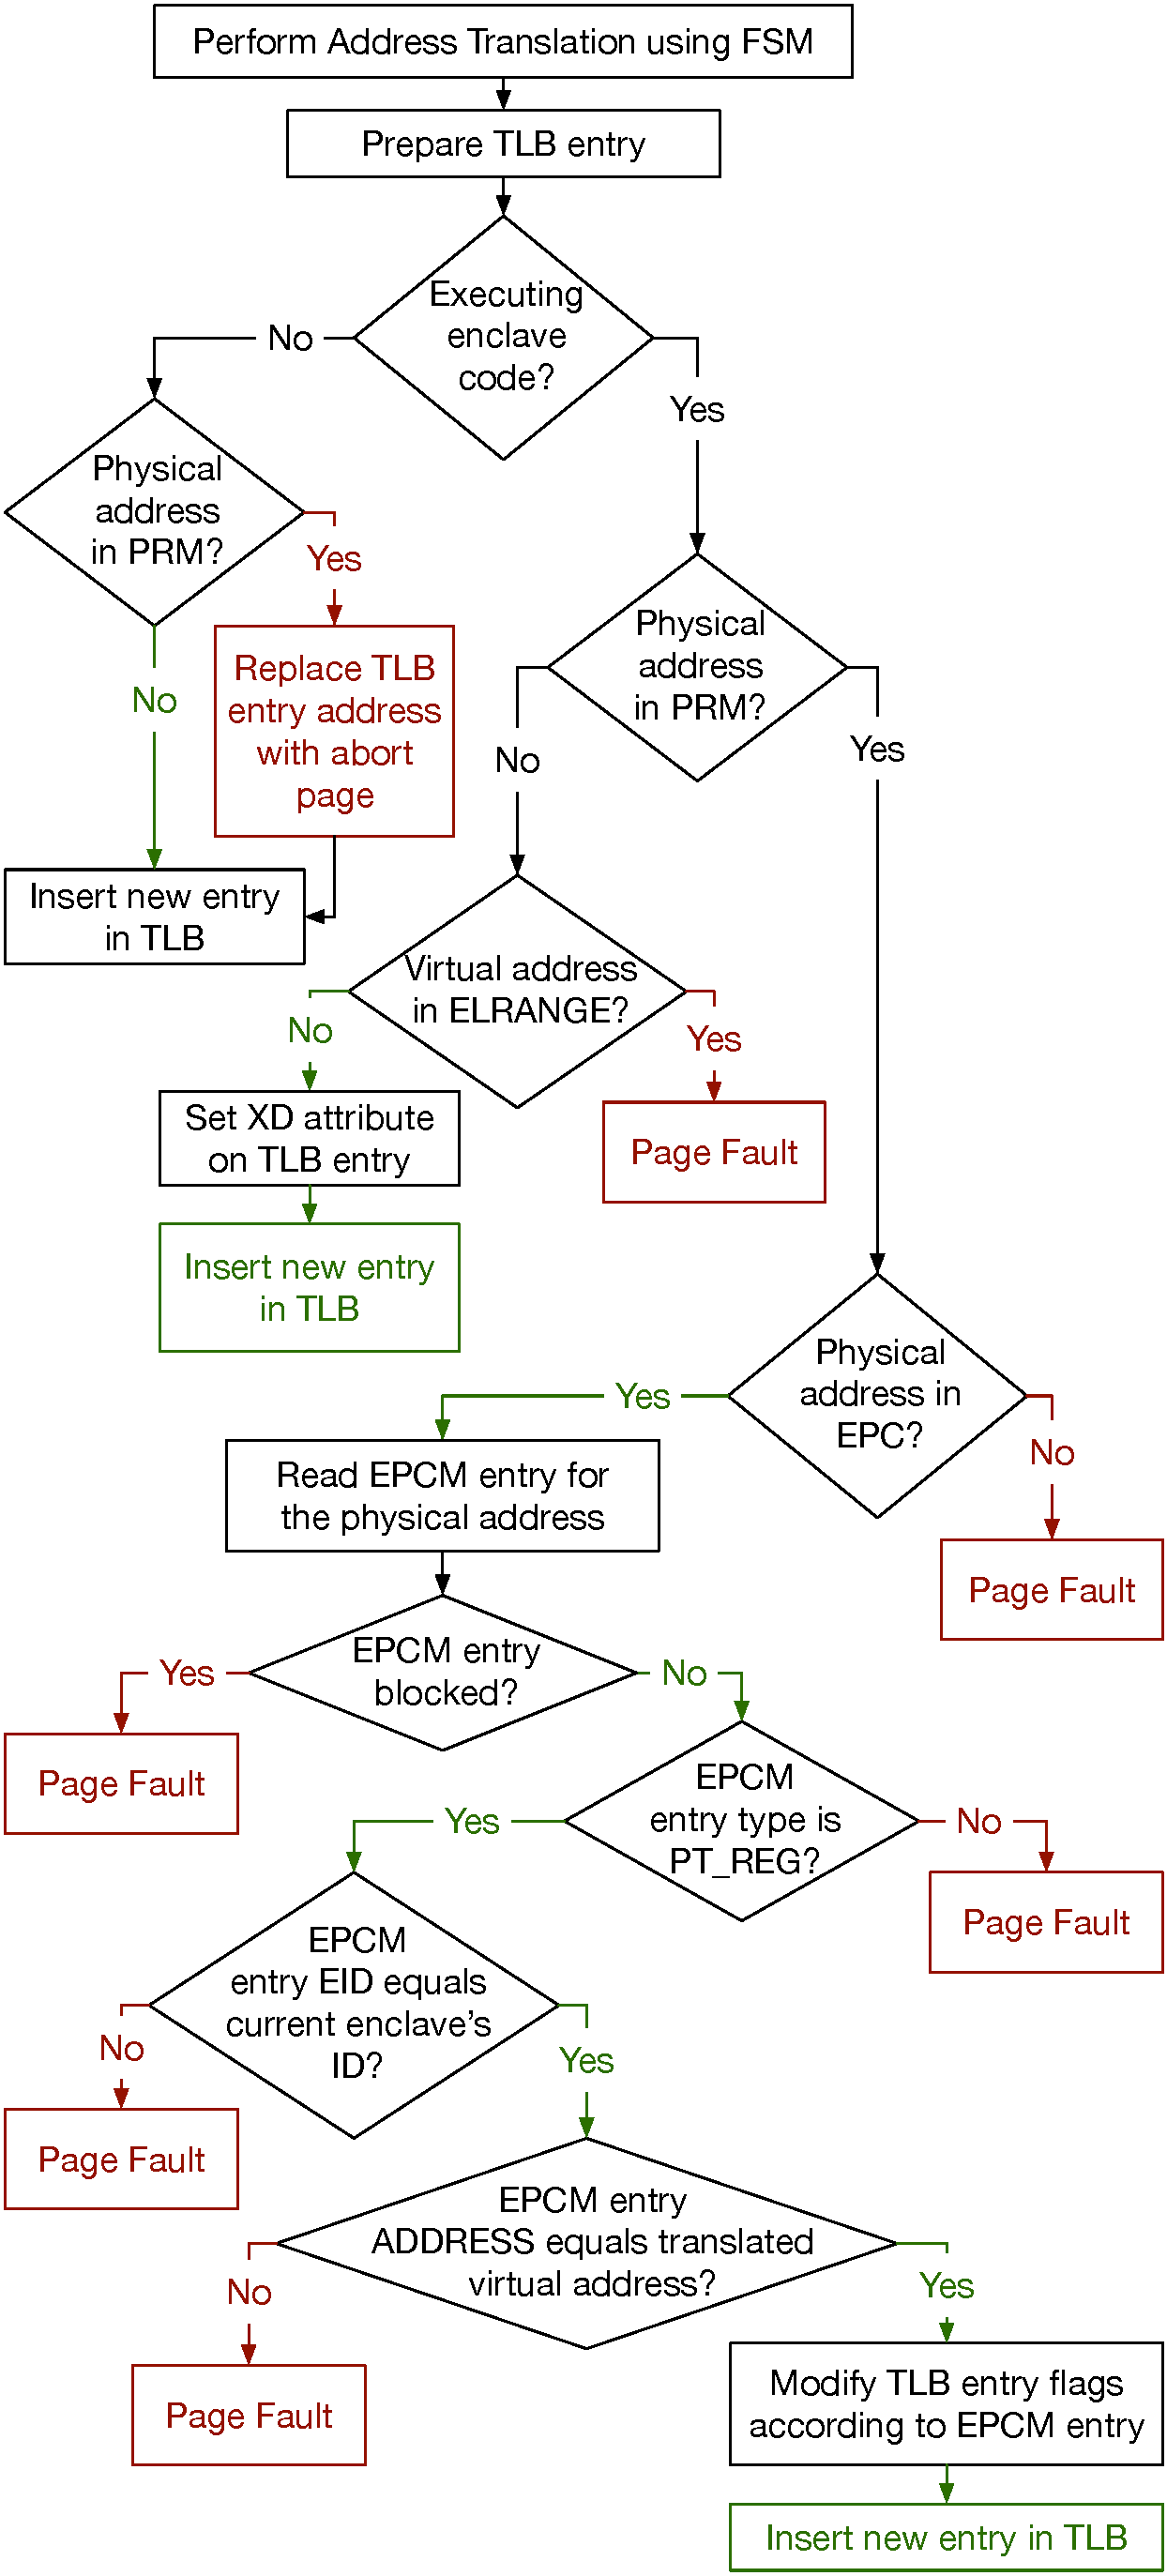
\includegraphics[width=85mm]{figures/sgx_tlb_miss_checks.pdf}
  \caption{
    SGX adds a few security checks to the PMH. The checks ensure that all the
    TLB entries created by the address translation unit meet SGX's memory
    access restrictions.
  }
  \label{fig:sgx_tlb_miss_checks}
\end{figure}



the CPU ensures\footnote{A mismatch triggers a general
protection fault (\#GP, \S~\ref{sec:faults}).} that the virtual address given
to the address translation process matches the expected virtual address
recorded in the page's EPCM entry, as shown in
Figure~\ref{fig:sgx_tlb_miss_checks}. This prevents the system software, which
manages the page tables and EPT, from modifying an enclave's virtual address
space in a manner that is inconsistent with the enclave author's expectations.


SGX's security revolves around maintaining the following
invariant. \textbf{At all times, a logical processor's TLB
entries can only map DRAM pages that can be accessed by the code executing on
the processor.} Specifically, when a logical processor is in enclave mode, its
TLB can include entries for the enclave's EPC pages, and for DRAM pages outside
the PRM. The TLB of a logical processor outside enclave mode must not include
any PRM entry.

Without any special measures, the invariant described above would be broken
when a logical processor exits an enclave, either via
\texttt{EEXIT}~(\S~\ref{sec:sgx_eexit}), or via an AEX~(\S~\ref{sec:sgx_aex}).
This is because enclave mode allows TLB entries that point to the currently
executing enclave's EPC pages, and these entries become disallowed the moment
the processor leaves enclave mode. The SGX implementation solves this problem
by flushing a logical processor's TLBs when it leaves enclave mode.
